\documentclass[12pt]{article}

% Any percent sign marks a comment to the end of the line

% Every latex document starts with a documentclass declaration like this
% The option dvips allows for graphics, 12pt is the font size, and article
%   is the style


\usepackage{url}
\usepackage{graphicx}
\usepackage{subcaption}

% These are additional packages for "pdflatex", graphics, and to include
% hyperlinks inside a document.
\pagenumbering{roman}

\addtolength{\oddsidemargin}{-.875in}
\addtolength{\evensidemargin}{-.875in}
\addtolength{\textwidth}{1.75in}

\addtolength{\topmargin}{-.875in}
\addtolength{\textheight}{1.75in}

% These force using more of the margins that is the default style

\begin{document}

% Everything after this becomes content
% Replace the text between curly brackets with your own

\title{Appendix}
\date{}

\maketitle

% This command causes the title to be created in the document
\section*{Data Analysis}

\subsection*{The Dataset}

Orders from Instacart are available in four .csv files: "orders.csv", "order\_products\_\_train.csv", "order\_products\_\_prior.csv" and "sample\_submission.csv". The key to understand the dataset and the train / test split is the orders table ("orders.csv").

Take for example User 1[Fig 1] , who happens to be a train user. User 1 has 10 prior orders, and 1 train order whose details are provided in "order\_products\_\_prior.csv" and in "order\_products\_\_train.csv" respectively.

\begin{figure}[!bp]
  \begin{subfigure}[b]{0.4\textwidth}
    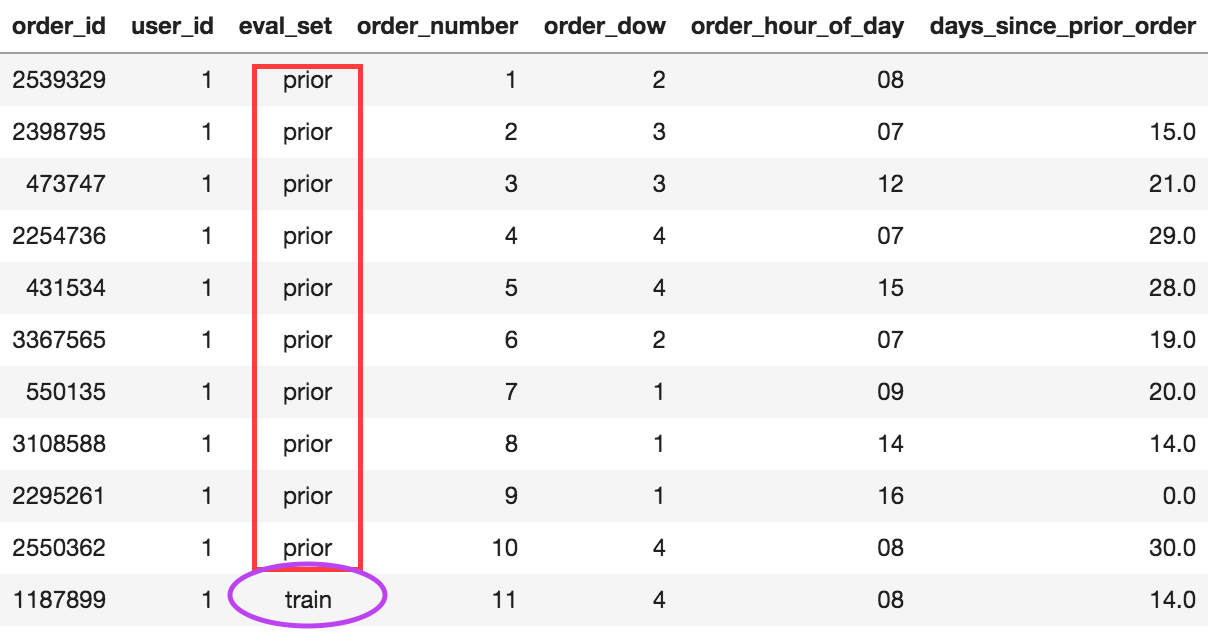
\includegraphics[width=\textwidth]{train_user.png}
    \caption{User 1}
    \label{fig:f1}
  \end{subfigure}
  \hfill
  \begin{subfigure}[b]{0.4\textwidth}
    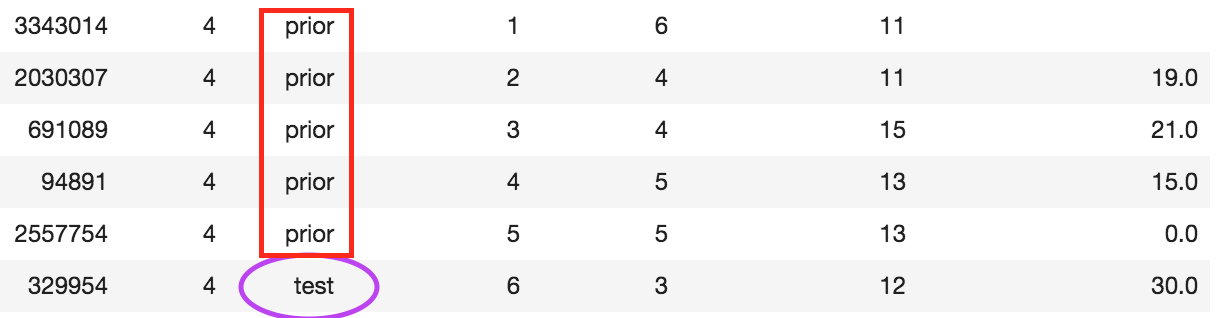
\includegraphics[width=\textwidth]{test_user.png}
    \caption{User 4}
    \label{fig:f2}
  \end{subfigure}
  \caption{Train/Test Split}
\end{figure}

Similarly, User 4 is a test user. He has 5 prior orders, and his 6th is a test order. Their details are available in "order\_products\_\_prior.csv" and "sample\_submission.csv" respectively.

Figure 2 is a glimpse at "order\_products\_\_prior.csv" when merged with three other .csv files that represent products, aisles and departments. The format of "sample\_submission.csv" and "order\_products\_\_train.csv" is exactly the same.

\begin{figure*}
	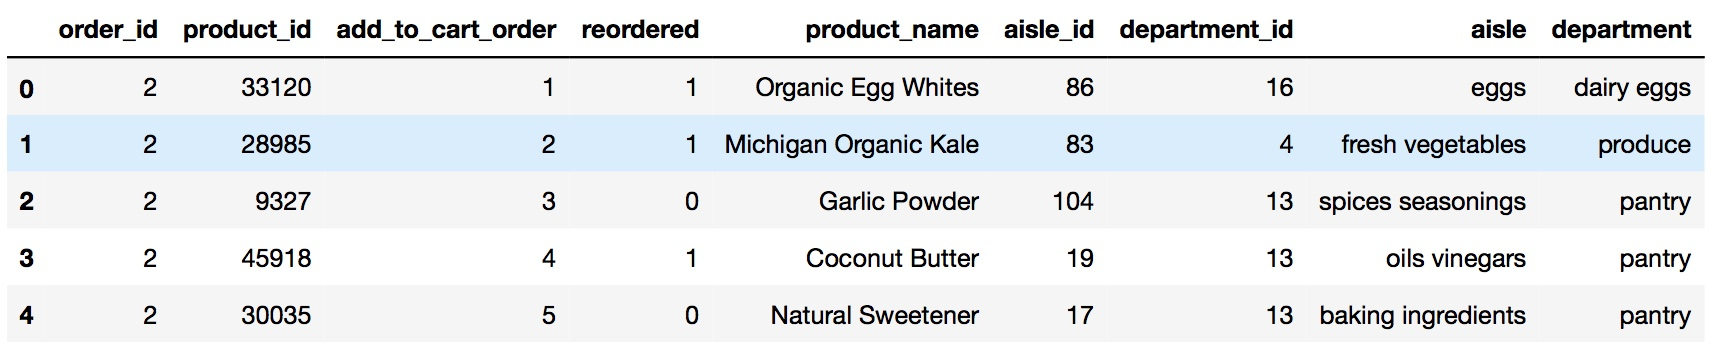
\includegraphics[scale=0.3]{prior_df_merged} \\
	\caption{Merged Prior Orders}
\end{figure*}


\subsection*{Exploration and Analysis}

\noindent
\textbf{How many orders have users placed?} \\
The below histogram validates the claim that 4 to 100 orders of a customer are given.
\begin{center}
	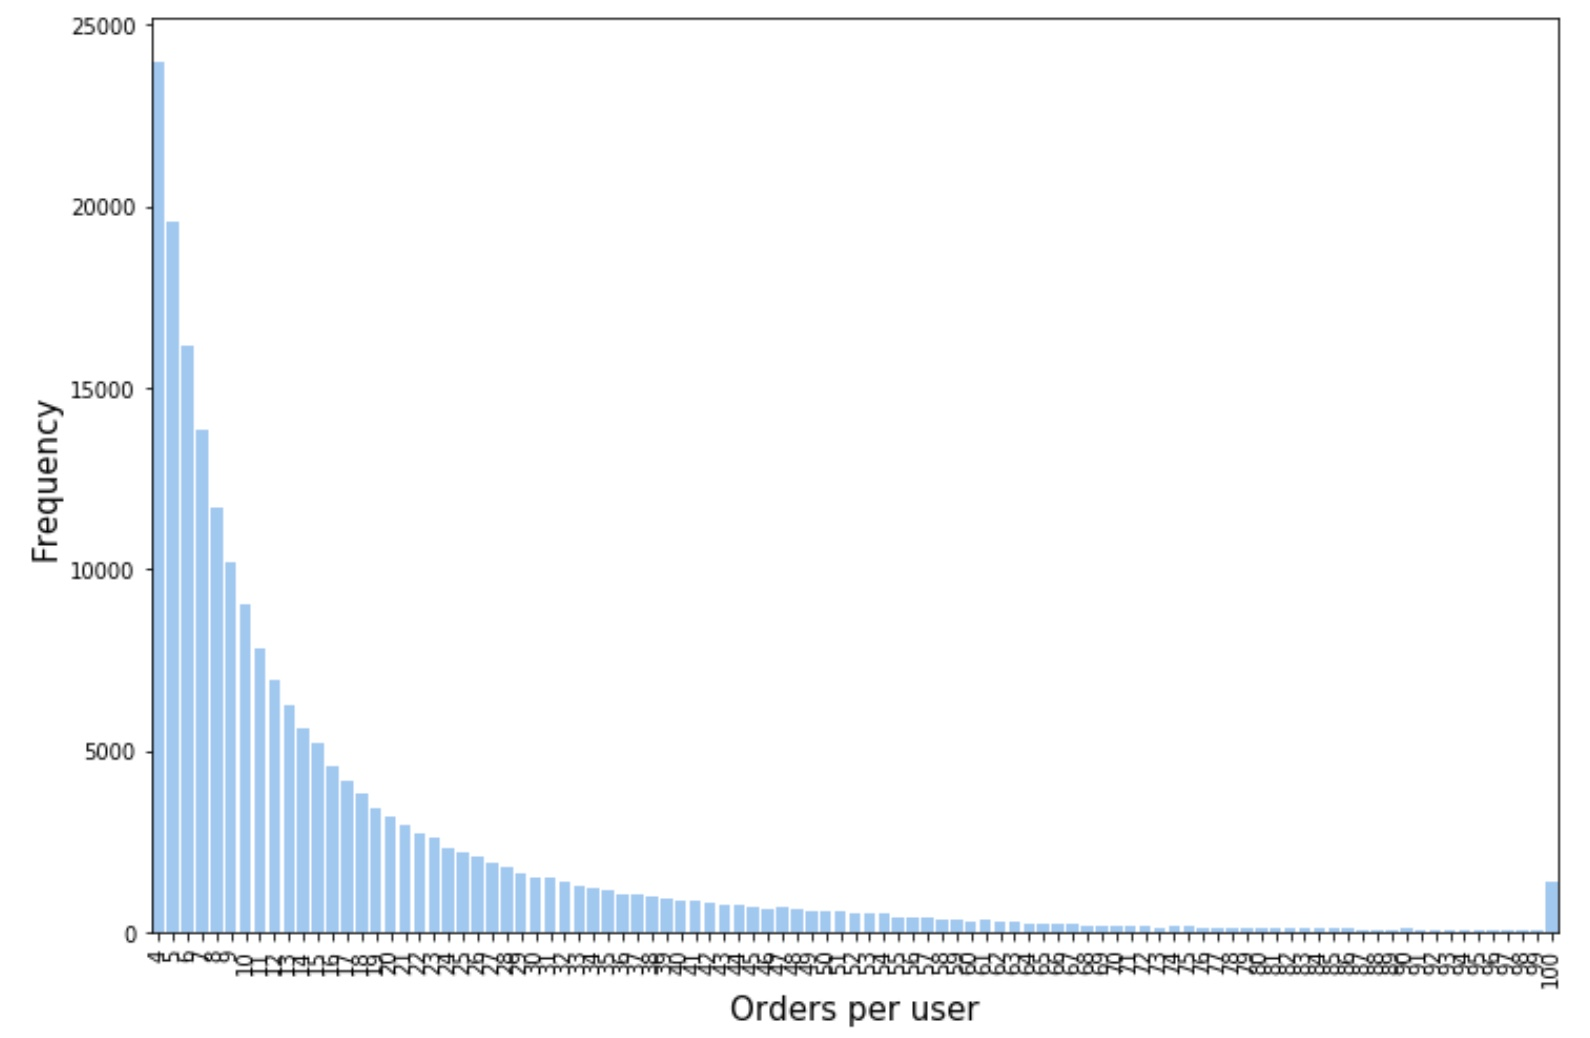
\includegraphics[scale=0.2]{order_user}
\end{center}


\noindent
\textbf{How many products does an order have??} \\
The "long tail" phenomenon is clearly visible here.
\begin{center}
	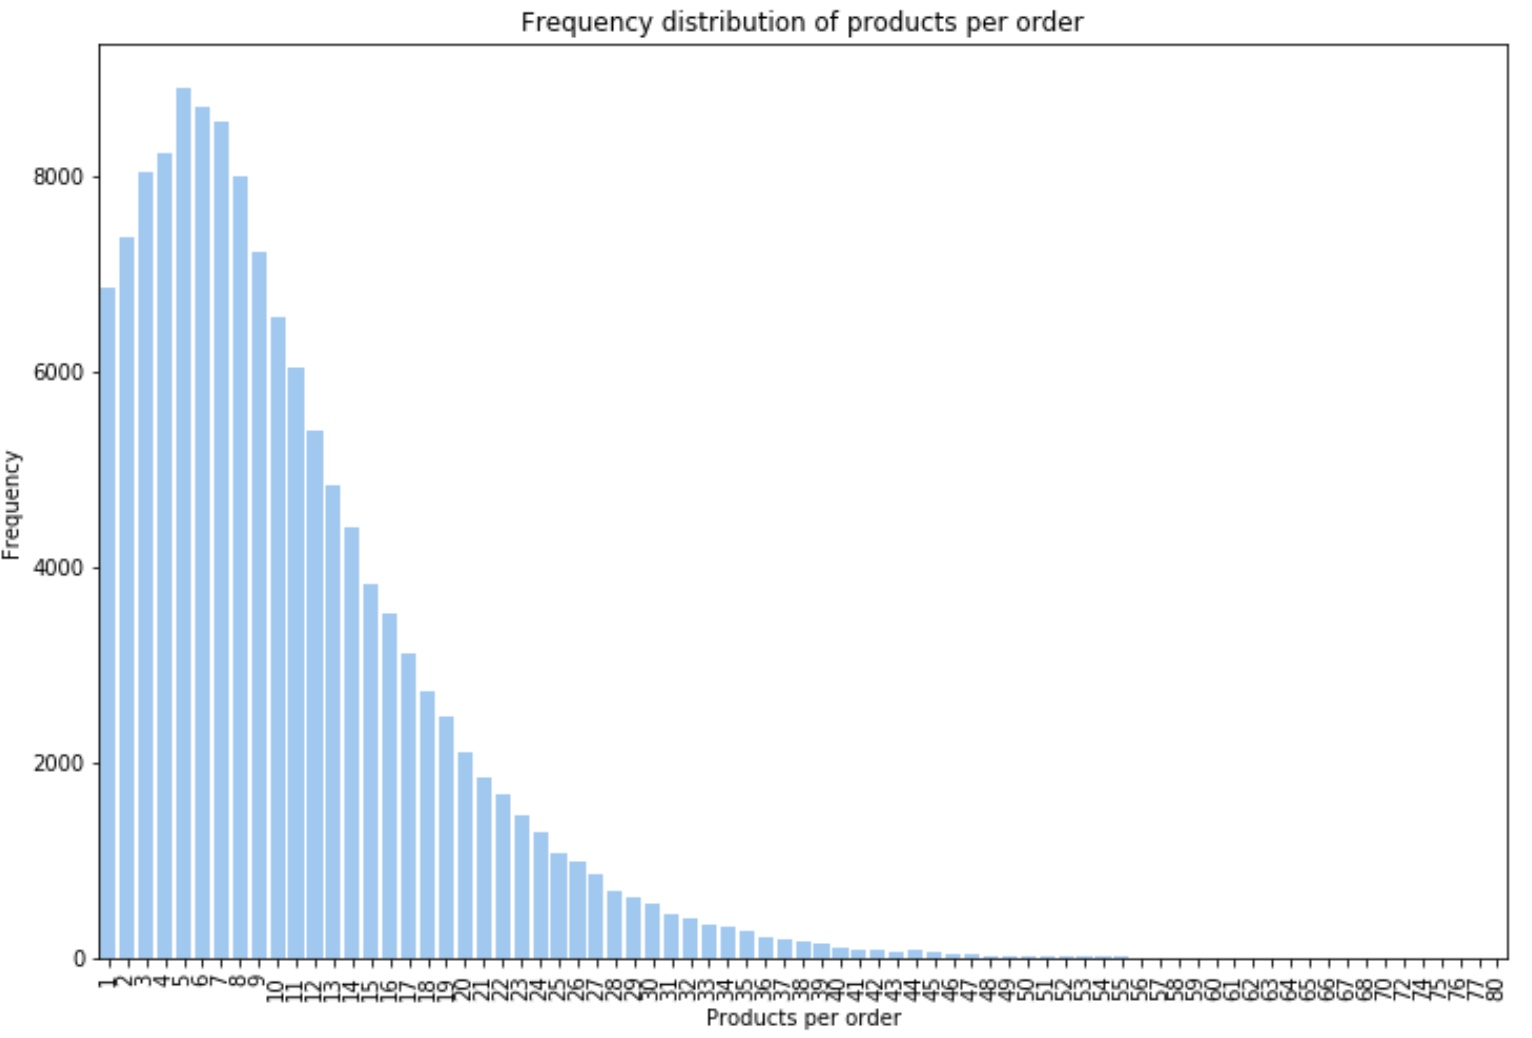
\includegraphics[scale=0.2]{train_products_order}
\end{center} 

\newpage
\noindent
\textbf{Does day of the week influence user order habits?} \\
There is a clear effect of day of the week. Most orders are on days 0 and 1. However, there is no information about which values represent which day, but, it's reasonable to assume they are weekends.
\begin{center}
	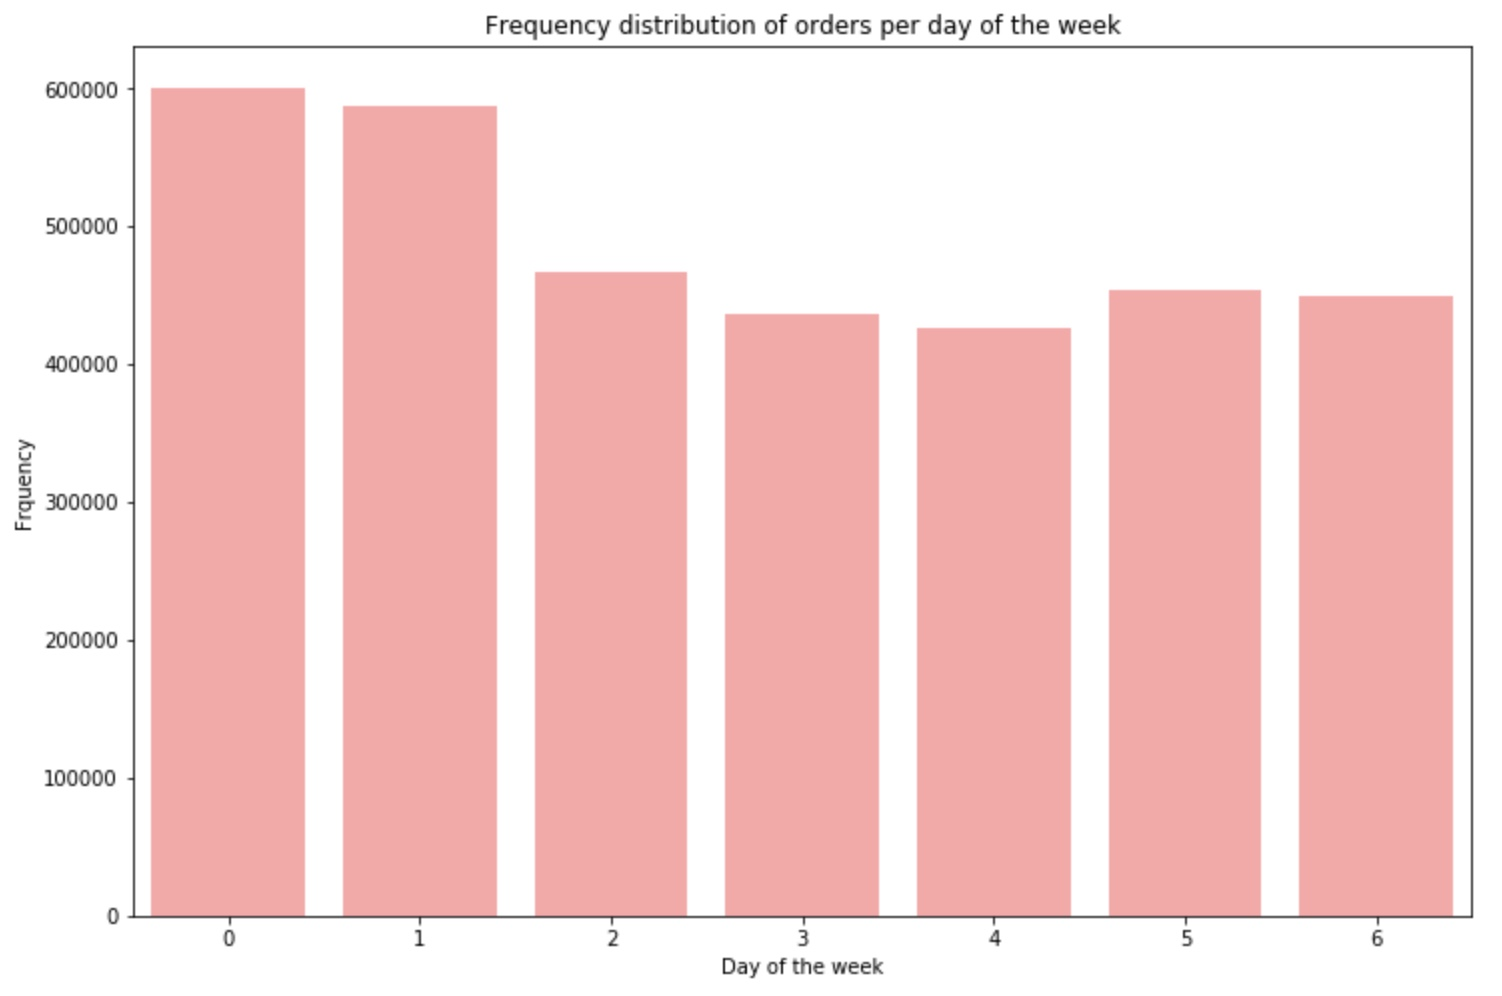
\includegraphics[scale=0.2]{order_dow}
\end{center}

\noindent
\textbf{Does time of day influence user order habits?} \\
There is a clear effect. Most of the orders are placed between 7.00 am and 10.00pm.
\begin{center}
	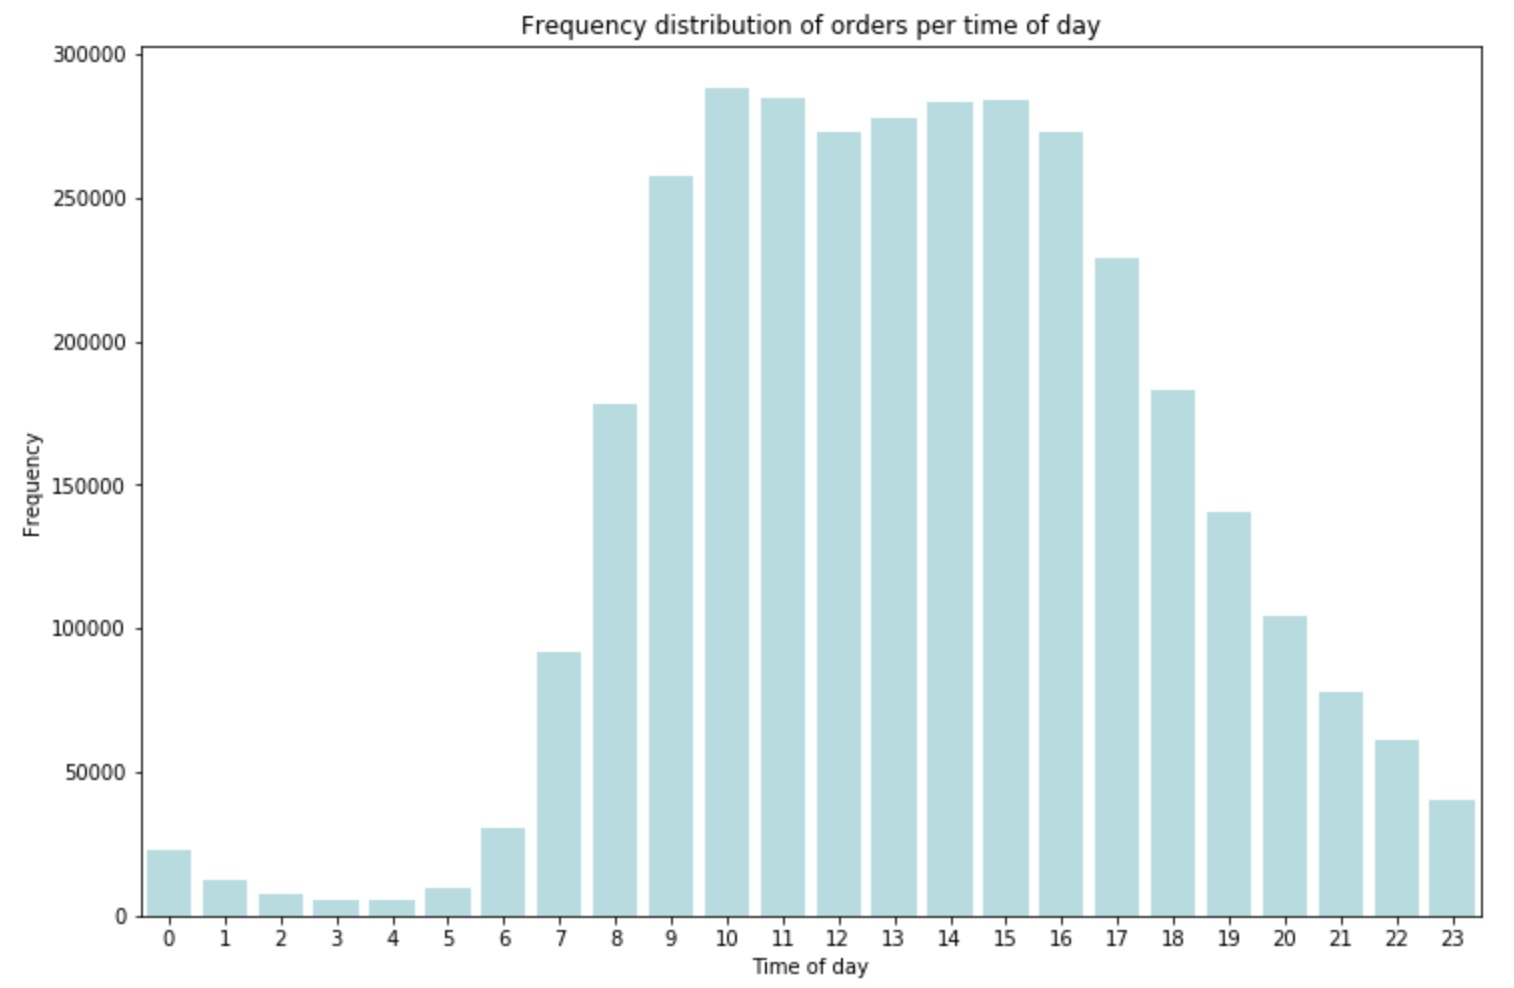
\includegraphics[scale=0.2]{order_tod}
\end{center}

\newpage
\noindent
\textbf{When do users reorder?} \\
Users seem to order on a weekly and monthly basis.
\begin{center}
	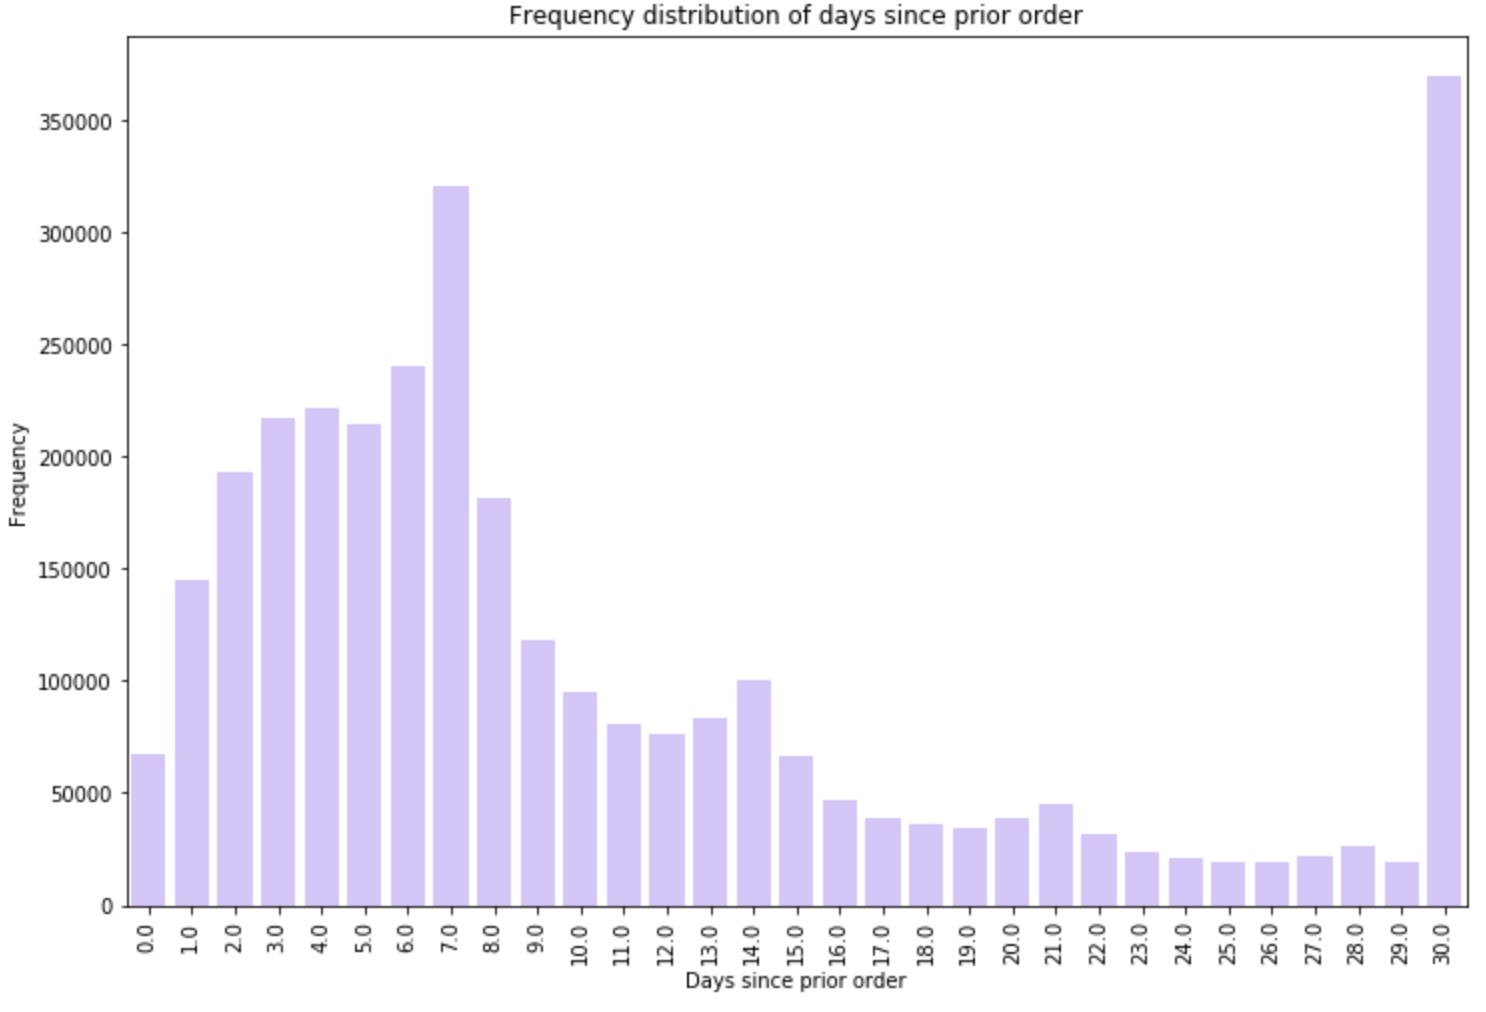
\includegraphics[scale=0.2]{days_since_prior_order}
\end{center}


\noindent
\textbf{What are the top 20 Products?} \\
\begin{center}
	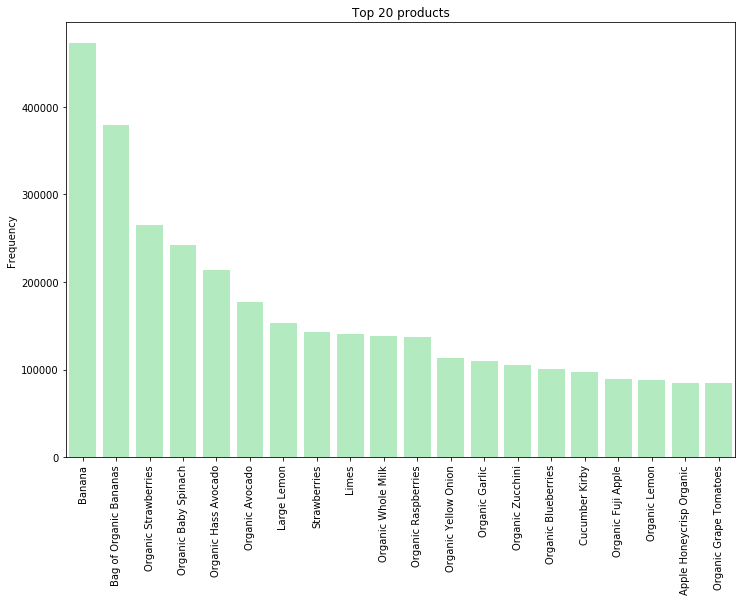
\includegraphics[scale=0.4]{top_20_products.png}
\end{center}


\end{document}





















